\documentclass[10pt]{article}

\usepackage{color}
\usepackage{listings}
\lstset{
language=C++,               	% choose the language of the code
basicstyle=\footnotesize,       % the size of the fonts that are used for the code
numbers=left,                   % where to put the line-numbers
numberstyle=\footnotesize,      % the size of the fonts that are used for the line-numbers
stepnumber=1,                   % the step between two line-numbers. If it is 1 each line will be numbered
numbersep=5pt,                  % how far the line-numbers are from the code
backgroundcolor=\color{white},  % choose the background color. You must add \usepackage{color}
showspaces=false,               % show spaces adding particular underscores
showstringspaces=false,         % underline spaces within strings
showtabs=false,                 % show tabs within strings adding particular underscores
frame=single,           		% adds a frame around the code
tabsize=2,          			% sets default tabsize to 2 spaces
captionpos=b,           		% sets the caption-position to bottom
breaklines=true,        		% sets automatic line breaking
breakatwhitespace=false,    	% sets if automatic breaks should only happen at whitespace
escapeinside={\%*}{*)},         % if you want to add a comment within your code
}

\usepackage{anyfontsize} %For arbitrary font sizes
\usepackage[T1]{fontenc}  
%\usepackage[margin=1cm]{geometry} % To make margins smaller
\usepackage{microtype}  % To improve hyphenation, justification etc...
\usepackage{pdfpages}
%\pgfpagesuselayout{2 on 1}[a4paper,border shrink=1mm]

%\usepackage[cm]{fullpage}
\usepackage[top=1.5cm, bottom=1.5cm, left=1.5cm, right=1.5cm]{geometry}

\usepackage{titlesec}
\titleformat{\section}{\large\bfseries}{\thesection}{2em}{}
\titleformat{\subsection}{\large\bfseries}{\thesubsection}{1em}{}

\pagestyle{myheadings}
\markright{Team Notebook (Perm SU: Meerkats)\hfill}

\begin{document}

\tableofcontents



\newpage
\section{Startup templates}
\subsection{template}
\lstinputlisting{../src/template.cpp}
\subsection{gvimrc}
\lstinputlisting{../src/gvimrc}



\newpage
\section{Graph Algorithms}
%\subsection{Kuhn Max Matching}
%\lstinputlisting{../src/kuhnMaxMatching.cpp}
\subsection{Dinic Max-Flow}
\lstinputlisting{../src/dinic.cpp}
\subsection{Hungary Algo}
\lstinputlisting{../src/assignmentHungary.cpp}
\subsection{Min Cut}
\lstinputlisting{../src/minCut.cpp}
\subsection{Bridges}
\lstinputlisting{../src/bridges.cpp}
\subsection{Cut Vertices}
\lstinputlisting{../src/cutVertices.cpp}
\subsection{Min-Cost Max-Flow}
\lstinputlisting{../src/minCostMaxFlow.cpp}
\subsection{Strongly Connected Components}
\lstinputlisting{../src/scc.cpp}
\subsection{2-SAT}
Problem: $(a ~ \vee ~ c) ~ \& ~ (a ~ \vee ~ !b) ~\& ~\ldots$

Edges: $(a ~ \vee ~ b)$ is equivalent to $(!a \Rightarrow b) \vee (!b \Rightarrow a)$

Solution: there is no solution iff for some $x$ $compID[x] = compID[!x]$, else see code below
\lstinputlisting{../src/2-sat.cpp}



\newpage
\section{Linear Algebra}
\subsection{Gauss Elimination}
\lstinputlisting{../src/gauss.cpp}
\subsection{Fast-Fourier Transform}
\lstinputlisting{../src/fft.cpp}
\subsection{Simplex}
\lstinputlisting{../src/simplex.cpp}



\newpage
\section{String Algorithms}
\subsection{Suffix Array}
\lstinputlisting{../src/suffixArray.cpp}
\subsection{Suffix Tree from Suffix Array}
\lstinputlisting{../src/suffixTree.cpp}
\subsection{Z-function}
\lstinputlisting{../src/zFunction.cpp}
\subsection{Suffix Automata}
\lstinputlisting{../src/suffixAutomata.cpp}
\subsection{Palindromes}
\lstinputlisting{../src/palindromes.cpp}
\subsection{Lyndon decomposition $\&$ Duval}
\lstinputlisting{../src/duval.cpp}



\newpage
\section{Modular}
\lstinputlisting{../src/modular.cpp}

\newpage
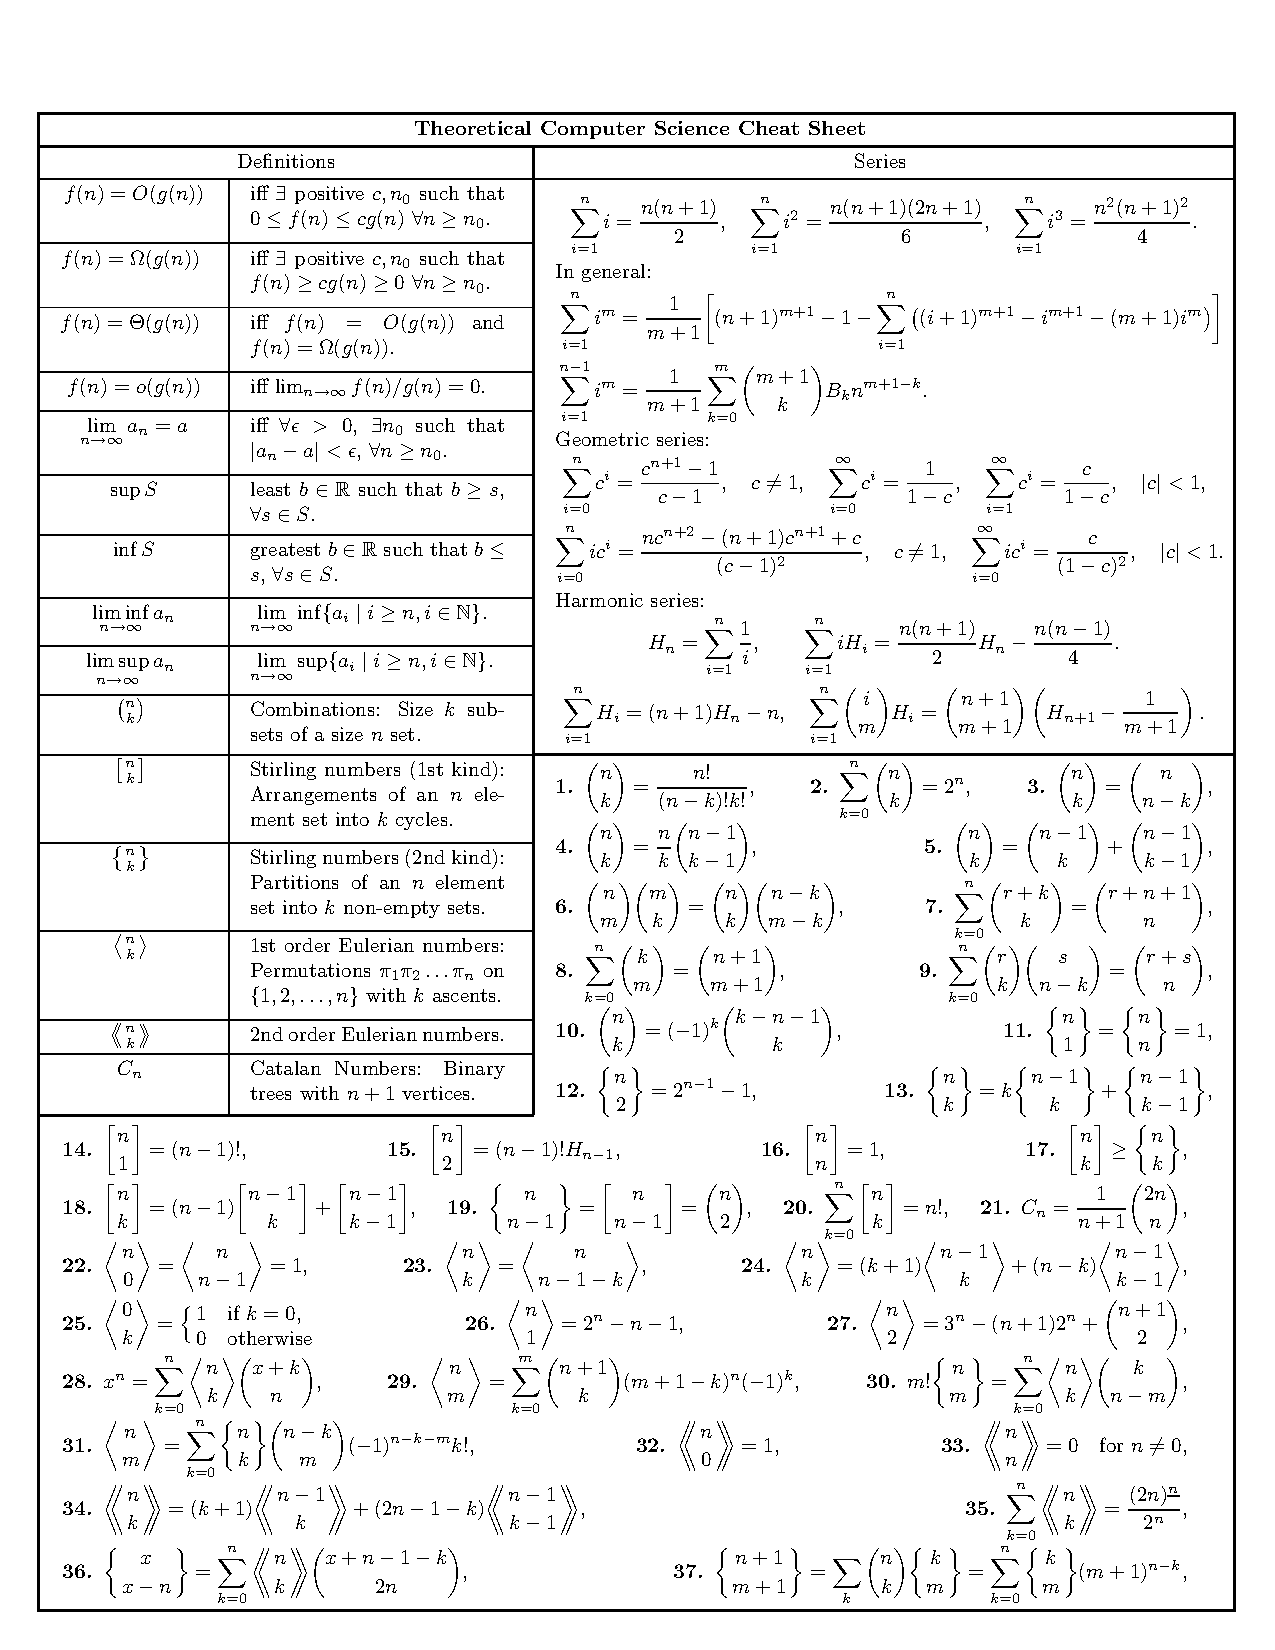
\includepdf[scale=0.95,pages={-}, pagecommand={\thispagestyle{myheadings}}]{../misc/cheatsheet.pdf}

\end{document}